\documentclass[conference]{IEEEtran}
\IEEEoverridecommandlockouts
% The preceding line is only needed to identify funding in the first footnote. If that is unneeded, please comment it out.
\usepackage{cite}
\usepackage{amsmath,amssymb,amsfonts, braket}
\usepackage{algorithmic}
\usepackage{graphicx}
\usepackage{textcomp}
\usepackage{xcolor}
\def\BibTeX{{\rm B\kern-.05em{\sc i\kern-.025em b}\kern-.08em
    T\kern-.1667em\lower.7ex\hbox{E}\kern-.125emX}}
\begin{document}

\title{Concise Insights into Quantum Machine Learning and Its Practical Uses}

\author{\IEEEauthorblockN{1\textsuperscript{st} Amir Arsalan Sanati}
\IEEEauthorblockA{\textit{Faculty of Computer Science and Engineering} \\
	\textit{Shahid Beheshti University}\\
Tehran, Iran \\
am.sanati@mail.sbu.ac.ir}
\and
\IEEEauthorblockN{2\textsuperscript{nd} Omid Reza Borzoei}
\IEEEauthorblockA{\textit{Faculty of Computer Science and Engineering} \\
	\textit{Shahid Beheshti University}\\
Tehran, Iran \\
o.borzoei@mail.sbu.ac.ir}
}

\maketitle

\begin{abstract}
Recent advancements in science and technology and emergence of the first digital computers, is considered as a new chapter in the book of technological achievements, which resulted in significant progress in various fields of industry and engineering. Simultaneously, with the improvement of quantum mechanics and discovering its properties, quantum computers emerged, showing remarkable computational power in comparison with digital computers. In our age, where we significantly use machine learning and processing large amounts of data is difficult and time-consuming for digital computers, the features of quantum computers can be a game-changer and greatly improve classical learning models. As a result, scientists and researchers are trying to utilize the power of quantum computations in order to create stronger and more accurate learning models. In this study, we will review the basic concepts of quantum computing, and with a focus on researches conducted in quantum machine learning, we will discuss the applications of this emerging field. Ultimately, with an overview and comparison on current quantum learning models, we will get to know the significant role of quantum computations in different fields of machine learning (like computer vision, natural language processing, reinforcement learning, cybersecurity, etc.) where the results promise notable improvements in the future of machine learning.
\end{abstract}

\begin{IEEEkeywords}
machine learning, quantum machine learning, quantum computing, entanglement, superposition, quantum mechanics, review, machine learning applications, quantum gates, quantum circuit
\end{IEEEkeywords}

\section{Introduction}
Machine learning is one of the pillars of artificial intelligence. Its basic concept includes creating appropriate models to extract hidden features or patterns from vast datasets and then make predictions based on the extracted features in order to solve some specific problems. Thanks to its exceptional problem-solving capabilities, ML outperforms humans in certain tasks such as image classification of large datasets \cite{b1}. However, with the increase of data in today's age of information, digital machine learning models have to process significantly large amount of information. Therefore, facing classical models with certain challenges \cite{b2},\cite{b3}. 

In recent years, advances in computational technology have opened our way to massive data processing. Quantum computing has shown that it can perform complex tasks much faster than classical computers \cite{b4}. The integration of quantum and machine learning algorithms leads to quantum machine learning technology, which is only achievable if we use real quantum computers \cite{b2}. Quantum machine learning is the use of quantum computing algorithms in machine learning programs. The term "quantum-enhanced machine learning" basically means Enhancing machine learning algorithms, to be able to run on quantum computers and perform operations on data. However, both the ideas of machine learning and quantum computing are still under development since their first appearance in recent years \cite{b5}. 

The way quantum computers work allows them to process data exponentially faster than conventional computers. Unlike digital systems whose operations only act on 1’s and 0’s, quantum computers perform calculations based on the probability of an object's state before measuring it \cite{b5}. In other words, it seems using quantum machine learning can greatly assist processing large amounts of data in machine learning tasks.

The purpose of this study is to get more familiar with this branch of technology and compare it with classical learning approaches. First, we will describe the history of quantum computers and quantum machine learning, then we will introduce some quantum phenomena which have led to the amazing power of quantum computation. After that, we will have an overview of the programming method of quantum computers (introducing a number of gates and quantum circuits), then we will examine the applications of quantum machine learning in different fields. And finally, we will compare digital and quantum models.

\section{History\textsuperscript{\cite{b8}}}
The idea of using quantum mechanics to perform calculations in new and exciting ways has been around since the emergence of this field.  Superposition and Entanglement principles can form the basis of a powerful form of computation.  The trick is to build a quantum system that we can easily manipulate and measure.  In 1979, a young physicist named Paul Benioff published a paper titled \textbf{"The computer as a physical system: A microscopic quantum mechanical Hamiltonian model of computers as represented by Turing machines"} at Argonne National Laboratory. In this paper, Benioff laid out the theoretical foundation for quantum computing and then suggested that such a computer could be built. He stated in his paper: "The whole computation process is described by a pure state evolving under the action of a given Hamiltonian. Thus, all the component parts of the Turing machine are described by states which have a definite phase relation to one another as the calculation progresses...The existence of such models at least suggests that the possibility of actually constructing such coherent machines should be examined.". Yuri Manin also expressed the main idea of quantum computing in his 1980 book "Computable and Non-Computable". In 1981, Richard Feynman, in a lecture, also touched on these topics and then specified the characteristics that a quantum computer must have to be efficient.

After these individuals pointed to the possibility of processing information in quantum systems, other scientists began to study algorithms that such systems could run. David Deutsch, a physicist at Oxford, published a paper in 1985. In this work, he detailed what a quantum algorithm might look like and predicted that one day it would be technologically possible to build quantum computers. After that, in 1992, Deutsch and Richard Jozsa presented an algorithm for a problem that could be solved on a digital computer in time complexity of $O(n)$ but could be solved on a quantum computer using the Deutsch-Jozsa algorithm in only $O(1)$. However, this algorithm had a problem: while the Deutsch-Jozsa algorithm demonstrated quantum supremacy, if small errors in calculations were allowed, both the classical and quantum versions could solve the problem in $O(1)$. A year later, in 1993, Umesh Vazirani and his student Ethan Bernstein, building on the Deutsch-Jozsa algorithm, presented another algorithm that could solve a different problem in $O(1)$ while that could be solved on digital computers in $O(n)$. Here, even if small errors in calculations were allowed, it didn't make the digital algorithm solve the problem faster, which indicated a definite advantage. In the same 1993 paper, they described a quantum version of the Fourier transform. This quantum Fourier transform would later prove to be a crucial component when Peter Shor developed his algorithm for factoring large numbers. After the work of Vazirani and Bernstein, Daniel Simon, in 1994, posed a problem that a quantum computer could solve significantly faster than a classical computer. To be more precise, Simon's algorithm has an upper bound of $O(n)$ on a quantum computer, but its classical counterpart has a lower bound of $\Omega(2^{\frac{n}{2}})$ steps, clearly demonstrating that the quantum algorithm is faster.

So far, all the research has been conducted without knowing whether a quantum computer could be built. Researchers simply assumed that if humans could build such a computer, their algorithms would outperform digital algorithms. Until Seth Lloyd, in a paper in the same year, outlined a method for building a quantum computer. He suggested that a system that sends pulses, such as electromagnetic pulses, to a unit, like an electrical circuit simulating an atom, could represent a quantum state.

In 1994, Peter Shor, building on the previous research of Deutsch-Jozsa, Bernstein-Vazirani, and Simon, was able to present a quantum algorithm for factoring large numbers into their prime factors. His algorithm broke the RSA encryption in theory and demonstrated that quantum computers could be so powerful to solve problems that classical computers. A few years later, in 2001, Isaac Chuang and his colleagues ran Shor's algorithm on a nuclear magnetic resonance system to factor the number 15. After Shor, other enhanced algorithms were also introduced. For example, Lov Grover presented a search algorithm that reduced the problem's time complexity from $O(n)$ to $O(\sqrt{n})$.

\begin{figure}[htbp]
\centerline{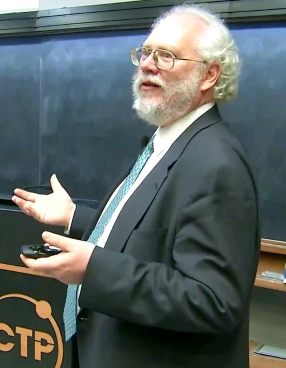
\includegraphics{peter_shor.png}}
\caption{Peter Shor}
\label{fig1}
\end{figure}

\begin{figure}[htbp]
	\centerline{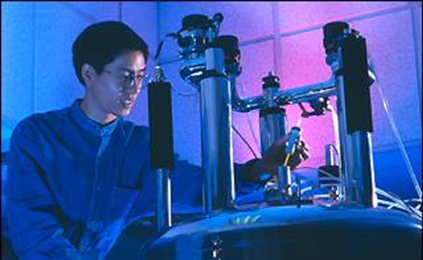
\includegraphics[scale=0.8]{chaung.png}}
	\caption{Isaac Chuang's Quantum Computer}
	\label{fig2}
\end{figure}

\section{Emergence of the Word “Quantum Machine Learning"}
The field of quantum machine learning (QML) is considered as a promising intersection between quantum computing and artificial intelligence, whose foundations can be traced back to early works on quantum algorithms and quantum information processing in the 1990s and 2000s. In 1996, Lov Grover developed a quantum algorithm for database search which was much faster than classical algorithms \cite{b9}. This work laid the groundwork for exploring the potential of quantum mechanics to improve machine learning tasks. During the next decade, researchers investigated ways to take advantage of quantum phenomena such as superposition and entanglement to improve the performance of machine learning algorithms \cite{b10}. In the 2010s, the field of QML gained significant momentum as advances in quantum hardware and the growing maturity of machine learning techniques converged. Foundational works such as the presentation of a quantum algorithm for solving linear equations \cite{b11} and the development of quantum enhanced neural networks \cite{b12} showed the potential of QML to outperform classical approaches in some problem domains. With the continuous development of quantum computing hardware, the integration of quantum mechanics and machine learning will open new opportunities to solve complex problems in areas such as optimization, simulation, and data analysis \cite{b13}. The word QML itself was used for the first time in 2013 by Lloyd, Mohseni and Rebentrost, and in 2014, Peter Wittek published a book about this subject under the same title \cite{b14}.

\section{The Power of Quantum Systems}
Quantum computing operates based on the postulates of quantum physics and utilizes the strange behaviors of subatomic particles to perform calculations faster and more efficiently \cite{b15}. In general, several properties of quantum mechanics are used in quantum computation, but two of the most important ones, which can almost be considered as the source of the powerfulness of quantum computers, are the principles of superposition and entanglement \cite{b15}, \cite{b16}, \cite{b16}, \cite{b18}. In this section, we will introduce these two principles along with some other principles and concepts of quantum mechanics and quantum computation to get a relative understanding of why quantum computers are powerful.

\subsection{Qubit}
Qubit (quantum bit) is the basic unit of information in some quantum systems, which is similar to bits in classical systems. Unlike classical systems, where a bit can only have one of two values, 0 or 1, a qubit can also be in two or more than two states simultaneously (which in qubits, we reduce these states into two states named as $\ket{0}$ and $\ket{1}$). Mathematically, a qubit is a unit vector in a two-dimensional Hilbert space \cite{b15}, \cite{b16}, \cite{b19}.

\begin{equation}
	\ket{\psi} = \alpha\ket{0} + \beta\ket{1} = \begin{bmatrix}
		\alpha \\
		\beta
	\end{bmatrix} \ \ \ \ \ \ \ \ \ \ \alpha, \beta \in C \label{eq1}
\end{equation}

where $|\alpha|^{2} +  |\beta|^{2} = 1$ and $\alpha$ and $\beta$ each represent the probability of the qubit being in the states of $\ket{0}$ and $\ket{1}$ after measurement ($\psi$ function is called wave function which expresses the state of a quantum bit in the form of probabilities). The difference between a classical bit and a quantum bit is shown in Fig.~\ref{fig3}.

\begin{figure}[htbp]
	\centerline{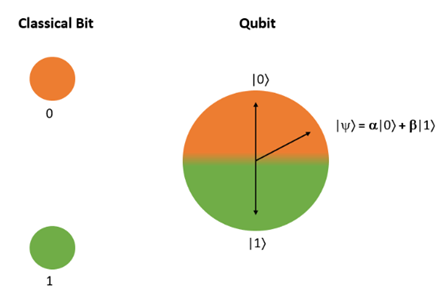
\includegraphics{difference.png}}
	\caption{Difference between classical bit and qubit \cite{b13}}
	\label{fig3}
\end{figure}

A problem with this model of representing qubits is that they cannot be visualized, because the coefficients $\alpha$ and $\beta$ are both complex numbers \cite{b20}. There’s another way of describing a qubit, which can visualize a qubit state and has various applications, known as Bloch sphere. Since the qubit coefficients are complex numbers, they can be rewritten as:

\begin{equation}
	\ket{\psi} = r_\alpha e^{i\phi\alpha}\ket{0} + r_\beta e^{i\phi\beta}\ket{1}
	\label{eq2}
\end{equation}
\begin{equation}
	\ket{\psi} = e^{i\phi\alpha}(r_\alpha \ket{0} + r_\beta e^{i(\phi_\beta - \phi_\alpha)}\ket{1})
	\label{eq3}
\end{equation}

In quantum mechanics, $e^{i\phi\alpha}$ is called "general phase", which has no effect on the measurement of the quantum state of a qubit (it can be ignored) \cite{b20}. Therefore, we will have:

\begin{equation}
	\ket{\psi} = r_\alpha \ket{0} + r_\beta e^{i\phi}\ket{1}
	\label{eq4}
\end{equation}

The value $(\phi_\beta - \phi_\alpha)$ is called "relative phase" which we replaced by $\phi$. Also, we restrict $\phi$ to be only in the interval $[0, \ 2\pi)$. On the other hand, the condition $|\alpha|^{2} + |\beta|^{2} = 1$ convinces us that $r_\alpha ^{2} + r_\beta ^{2} = 1$. This equation can be shown on the first quadrant of the unit circle (Fig.~\ref{fig4}). Therefore, we obtain:

\begin{equation}
	r_\alpha = \cos\left(\frac{\theta}{2}\right), r_\beta = \sin\left(\frac{\theta}{2}\right), 0 \le \theta \le \pi
	\label{eq5}
\end{equation}

Therefore, the quantum state of a qubit can be rewritten as follows, which consists of only two variables $\phi$ and $\theta$:

\begin{gather}
	\ket{\psi} = \cos\left(\frac{\theta}{2}\right)\ket{0} + \sin\left(\frac{\theta}{2}\right)e^{i\theta}\ket{1}
	\\
	\theta \in \left[0, \ \pi\right)
	\\
	\phi \in \left[0, \ 2\pi\right)
	\label{eq6}
\end{gather}

Therefore, we were able to change the state of a qubit from a four-dimensional value (two complex numbers) to an equivalent two-dimensional value which can be representable. By representing variables obtained earlier on spherical coordinates, the Bloch sphere appears \cite{b20}, \cite{b21} (Fig.~\ref{fig5}).

\begin{figure}[htbp]
	\centerline{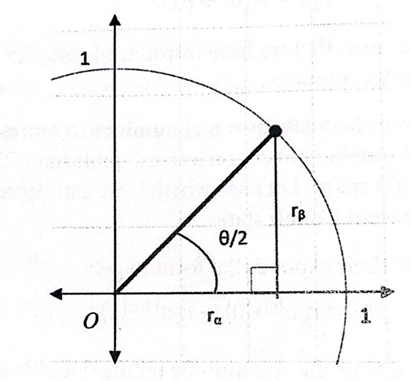
\includegraphics[scale=0.8]{circle.png}}
	\caption{Representation of $r_\alpha$ and $r_\beta$ on the first quadrant of the unit circle \cite{b14}}
	\label{fig4}
\end{figure}

\begin{figure}[htbp]
	\centerline{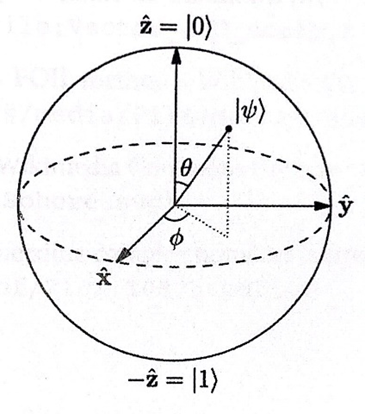
\includegraphics[scale=0.8]{block.png}}
	\caption{The Bloch Sphere \cite{b14}}
	\label{fig5}
\end{figure}

\subsection{The Principle of Superposition}
Qubits can be in a superposition of states $\ket{0}$ and $\ket{1}$, meaning it can be at both  $\ket{0}$ and $\ket{1}$ at the same time. Thus, only one quantum bit is sufficient to store a value worth two classical bits, similarly four classical bits are equivalent to two quantum bits. Generally, $2^{n}$ classical bits can be stored in $n$ quantum bits \cite{b19}. However, when the qubit state is measured, the overlap between states collapses and the value of the quantum bit will be a possible result of either 0 or 1. That is, with the probability $P\left(\ket{0}\right) = |\alpha|^{2}$  , the value of the qubit after measurement is zero, and with the probability $P\left(\ket{1}\right) = |\beta|^{2}$, this value will be one. This unique property of quantum reduces the space required for storage and can enable the parallelization of calculations \cite{b15}, \cite{b19}.

\subsection{The Principle of Entanglement}
Entanglement is an observed physical phenomenon in which a pair or group of qubits can be in a shared quantum state in such a way that each of them cannot be described independently, regardless of the distance between them. Any measurement on one, instantly identifies the result of measurement for the other \cite{b15}. This means that the state of one qubit is somehow connected to the state of other qubits. Therefore, this feature helps qubits to be correlated with each other despite being separated by large physical distances \cite{b19}.

The interesting point to note, is that since the entangled qubits have correlated states (Fig.~\ref{fig6}), when the state of one qubit changes, independent of the physical distance, the state of the rest of the qubits also changes instantly (with a relation which is known to us and can be engineered). Therefore, if we consider the change of state as calculation, by performing a calculation on one qubit, we have performed approximately $2^{n}$ other calculations simultaneously. For example, the representation of the quantum state for two entangled qubits is as follows:

\begin{gather}
	\ket{\psi} = \alpha_{00} \ket{00} + \alpha_{01} \ket{01} + \alpha_{10} \ket{10} + \alpha_{11} \ket{11} \\
	|\alpha_{00}|^{2} + |\alpha_{01}|^{2} + |\alpha_{10}|^{2} + |\alpha_{11}|^{2} = 1 \\
	P\left(\ket{00}\right) = |\alpha_{00}|^{2}, P\left(\ket{01}\right) = |\alpha_{01}|^{2}, ...
	\label{eq11}
\end{gather}

\begin{figure}[htbp]
	\centerline{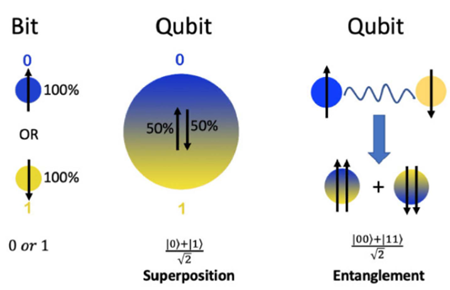
\includegraphics[scale=0.9]{ent.png}}
	\caption{An illustration of Superposition and Entanglement \cite{b16}}
	\label{fig6}
\end{figure}

\subsection{The No Cloning Theorem}
This theorem states that it is not possible to create an identical copy of an arbitrary unknown quantum state. It helps to infer that once a measurement is performed, it is not sure to get the same information after another measurement being performed on an already measured state \cite{b19}. Thus, in contrast to classical computing, where digital data can be copied easily, quantum information cannot be copied to other qubits. While this has an impact on algorithm approach and design, this property is of particular use in cryptography \cite{b15}.

\subsection{Wave Function Collapse}
Quantum measurement depends on the wave function collapse. Due to interaction with the external world, the wave function which is initially in a superposition of several states gets reduced to a single state. This leads to measurement of a quantum state which is probabilistic in nature \cite{b19}. This represents a great challenge in the implementation of a practical quantum computer, as it requires a pristine environment and is vulnerable to even the slightest external environmental disturbance \cite{b19}.

\subsection{Quantum Gates}
As in classical computers, we have digital gates that convert input digital values into desired output values, forming the basis of digital computer calculations. In quantum computers we also have quantum gates (Table~\ref{table1}). Quantum gates are quantum operations which are used to convert a qubit from an input state to a desired output state. Once a quantum gate is applied it is expected that the norm of the state vector maintains unity i.e., the sum of the squares of amplitudes should be equal to one. These gates are reversible in nature. These quantum gates are used as a basic building block in machine learning to perform computations \cite{b19}. Quantum gates are mathematically unitary matrices that are applied to an input vector and output a new vector. In other words, quantum gates are linear transformations which map the input state vector to the output state vector. For example, if we apply the Pauli-X gate on state $\ket{1}$ the result is as follows:
\begin{gather}
	\ket{\psi} = \ket{1} = \begin{bmatrix}
		0 \\
		1
	\end{bmatrix}, X = \begin{bmatrix}
	0 & 1 \\
	1 & 0
	\end{bmatrix} \\
	\ket{\psi_{out}} = X\ket{\psi} = \begin{bmatrix}
		0 & 1 \\
		1 & 0
	\end{bmatrix} \times \begin{bmatrix}
	0 \\
	1
	\end{bmatrix} = \begin{bmatrix}
	1 \\
	0
	\end{bmatrix} = \ket{0}
\end{gather}

\begin{table}[htbp]
	\caption{Quantum Gates \cite{b10} (Gates 7 and 8 are used for 2 Entangled Qubits)}
	\centerline{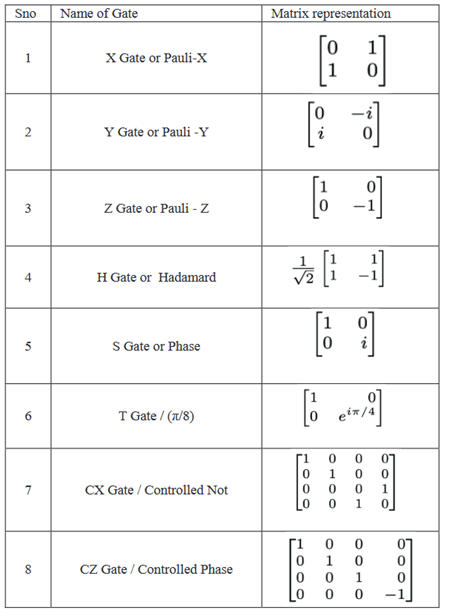
\includegraphics[scale=0.9]{gates.png}}
	\label{table1}
\end{table}

\subsection{Quantum Circuits}
Just like digital integrated circuits that include a network of classical (CMOS) gates which are applied respectively to input and result the output, quantum circuits also consist of quantum gates with specific order that are applied to a number of input qubits and perform a quantum algorithm (Fig.~\ref{fig7}).The process of running a quantum algorithm is as follows: first, the input qubits are initialized to a desired state, then quantum gates are applied in a specific sequence, and finally, after the algorithm is finished, the states of qubits are measured (right side of Fig.~\ref{fig7}).

\begin{figure}[htbp]
	\centerline{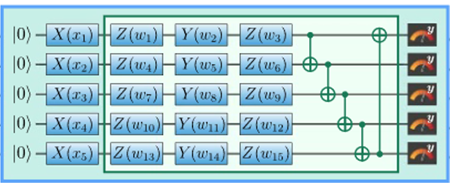
\includegraphics[scale=0.9]{qc.png}}
	\caption{An example of a quantum circuit used in a quantum neural network for image classification task \cite{b17}}
	\label{fig7}
\end{figure}

Therefore, by using quantum gates and quantum circuits, arbitrary algorithms (including algorithms related to machine learning) can be implemented. Algorithms which leverage the supremacy of the quantum realm.

\section{Integration of Quantum Computer and Machine Learning}
In the first step, quantum machine learning is achievable via hybrid quantum-classical models. Data of quantum origin can be represented and generalized using a quantum model. Quantum models cannot generalize quantum data using purely quantum processors because these processors are still small and error prone. As we are currently in the \textbf{era of noisy intermediate-scale quantum computers (NISQ)} and in this era, computers are not large and accurate enough, which makes the implementation of quantum algorithms difficult \cite{b31}. To be more efficient, NISQ processors must cooperate with traditional processors that form a quantum-classical model. A quantum neural network can do computations with fewer steps, fewer qubits, and shorter calculation times \cite{b5}. In fact, the term "quantum machine learning" refers to traditional machine learning techniques which are used on data produced by experiments conducted. The study of methodological and structural similarities between certain physical systems and learning systems, in particular neural networks, is known as quantum machine learning. For instance, classical deep learning may leverage some mathematical and numerical techniques from quantum physics, and vice versa \cite{b5}. The workflow of ML and QML can be seen in figure (Fig.~\ref{fig8}):

\begin{figure}[htbp]
	\centerline{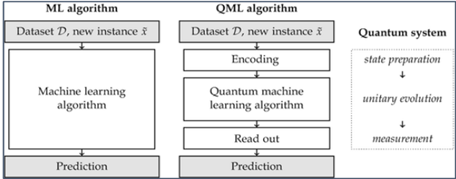
\includegraphics[scale=0.9]{qmlalgo.png}}
	\caption{The workflow of ML and QML \cite{b5}}
	\label{fig8}
\end{figure}

QML consists of different techniques and QML techniques are classified into four classes, namely CC, CQ, QC, and QQ as shown in the table (Table~\ref{table2}). The classification is based on whether the data is in the quantum or the classical form and whether the computation is in the quantum or the classical form \cite{b24}.

\begin{table}[htbp]
	\caption{Classification of QML \cite{b24}}
	\centerline{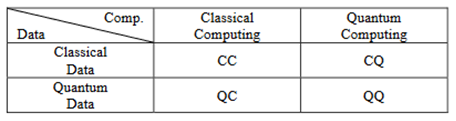
\includegraphics[scale=0.9]{class.png}}
	\label{table2}
\end{table}

As an example, we describe the class QQ. In the quantum data with quantum computing (QQ) class, techniques within it are considered to directly use quantum computation for processing quantum data, as well as for training ML models and for running the trained models. For example, a quantum computing device is employed to simulate complex quantum systems, and the simulated quantum data is directly analyzed with quantum ML models to obtain analytical results \cite{b24}. Depending on the desired capability and type of data set we have, we can choose a suitable quantum machine learning model.

\section{Applications of Quantum Machine Learning}
Quantum machine learning models can appear with better speed and performance in all fields where conventional machine learning models are used today. Furthermore, in many cases where classical models suffer from low efficiency, quantum models can be used instead. In this section we will discuss some of the applications of quantum models.

\subsection{Better Performance in Comparison to Current Models}
One of the applications of classical models nowadays is prediction of cancer, stroke, etc., which are often highly accurate. But the accuracy can be increased even higher by using quantum models. For example, we can refer to the model made by Singh, Swetapadma and Pettnik, whose quantum enhanced model was able to record 4.7\% better test time accuracy than the classical model, and its accuracy was 6.8\% better during training \cite{b1}. Another example is A model developed to detect COVID-19 from the sound of cough. This model was built at Arizona State University and trained on quantum computers with different numbers of qubits and with different algorithms \cite{b25}. The results can be seen in the table below.

\begin{table}[htbp]
	\caption{Results of the COVID-19 Quantum Model \cite{b25}}
	\centerline{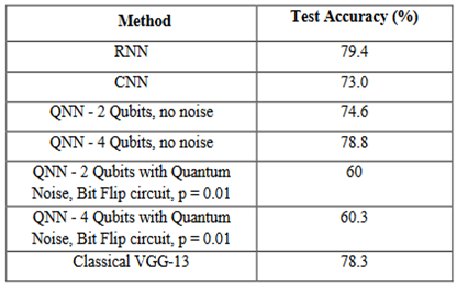
\includegraphics[scale=0.85]{covid.png}}
	\label{table3}
\end{table}

In the table above, it can be seen that the quantum model with only 4 qubits has reached 78.8\% accuracy, which is higher than the classical VGG-13 model. Although the accuracy of quantum models is higher, it is extremely challenging to achieve quantum computers because they are currently very expensive \cite{b25}.

\subsection{Quantum Natural Language Processing}
A group of researchers in 2021 proposed a protocol based on quantum long short term memory (Q-LSTM, combination of Quantum computing and LSTM networks) for Q-NLP to perform various tasks in general but specifically for translating a sentence from English to Persian. Then, they generalized their method to use quantum circuits of sentences as an input for the Q-LSTM cell. This way, they proposed a QNLP model which was able to translate sentences in different languages \cite{b26}. In addition to that, a "meaning-aware" algorithm has been developed by applying a natural language processing algorithm on quantum computing. Although key techniques in quantum computing nowadays include search problems, quantum annealing, machine learning, quantum analysis simulation, and post-quantum cryptography, the proposed model combines other elements. Meaning awareness refers to the ability of the computer to understand both individual letters and the complete sentence \cite{b27}. In this year also, a new network architecture called Quantum Self-Attention Neural Network was introduced, which specifically implemented self-attention mechanisms in quantum neural networks. This model demonstrated better performance than the best existing QNLP models and is also resistant to low-level quantum noise \cite{b28}.

\subsection{Quantum Reinforcement Learning}
Recent advances in classical reinforcement learning (RL) and quantum computation point to a promising direction for performing RL on a quantum computer \cite{b32}. In that regard, many researchers have focused their effort on the subject. For example, Lokes et al. implemented a deep reinforcement learning quantum network in their article and tested it in the frozen lake environment. Their findings showed that the quantum model not only converged faster but also reduced the number of required parameters, with the ratio decreasing compared to classical models \cite{b33} (Table~\ref{table4}). Another group has focused on designing quantum models for reinforcement learning based on quantum photonics (a type of quantum computer where qubits are formed by photons). The advantage of using quantum photonics is that this platform allows the model to make decisions at the speed of light and is also energy-efficient in information storage \cite{b34}. Another group, noting that the limiting factor in quantum reinforcement learning is the number of qubits, has proposed a model for managing high-dimensional input space (dimensions higher than the number of qubits). They tested their model in a mini-grid environment and found that this quantum model could find the correct solution. They also proposed an encoding mechanism which is able to reduce the number of parameters to the scale of \textbf{log(n)} where n is the number of input dimensions \cite{b32}.

\begin{table}[htbp]
	\caption{The Number and the Order of Parameters Used by the Classical Q-Learning and Quantum Approaches \cite{b33}}
	\centerline{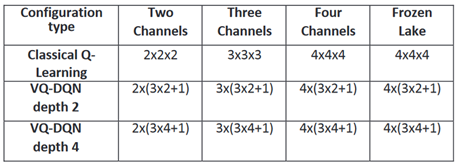
\includegraphics[scale=0.85]{qrl.png}}
	\label{table4}
\end{table}

\subsection{Image Processing and Computer Vision}
In the field of computer vision, particularly image classification, promising research has been conducted. Xiong and his colleagues presented a hybrid quantum-classical model (Fig.~\ref{fig9}) and tested it on the MNIST and CIFAR-10 datasets, achieving a model that was faster and more accurate than its classical counterpart \cite{b36}. Another group proposed a different hybrid model that achieved an accuracy of 99.21\% on the MNIST data, while using only one-eighth of the parameters of a classical model. They also tested their model on MedicalMNIST (99\% accuracy) and CIFAR-10 (82\% accuracy). Furthermore, they introduced a quantum convolutional layer and demonstrated that its performance matched that of its classical equivalent while using only one-fourth of the trainable parameters \cite{b37}.
\begin{figure}[htbp]
	\centerline{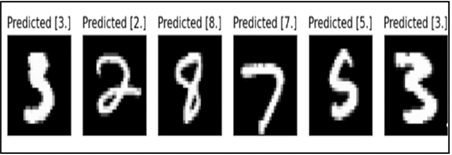
\includegraphics[scale=0.9]{qcnn.png}}
	\caption{Test result of Xiong’s model \cite{b36}}
	\label{fig9}
\end{figure}

\subsection{Autonomous Vehicles}
With the rise of autonomous vehicles (AVs), the number of self-driving vehicles has increased in recent years and vehicular computing (VC) was actively used to ensure road safety by controlling AVs. However, the recent escalation in demand for a massive scale vehicle network has prevented VC from achieving its purpose. To overcome this problem, a framework which combined VC and federated learning (FL) was proposed. Although the vehicular FL was initially effective, it also faced challenges as the excessive increase in the amount and size of data generated by AVs and the serious threat of data leakage have severely degraded the performance of vehicular FL. Thus, quantum computing was exploited to further improve on the preexisting FL and proposed dynamic quantum federated learning (DQFL). Kim, in his work proposed the application of DQFL to AV scenarios. He was the first one to study the application and investigate the effectiveness of the model in controlling the AVs under real-life constraints \cite{b38}.

\subsection{Health Care}
In the field of health and hygiene, many applications of QML can be mentioned, which are shown in the figure (Fig.~\ref{fig10}).

\begin{figure}[htbp]
	\centerline{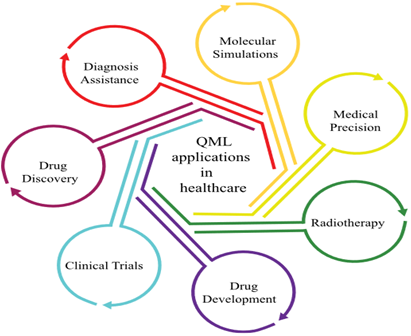
\includegraphics[scale = 0.9]{health.png}}
	\caption{Applications of QML in Health Care \cite{b29}}
	\label{fig10}
\end{figure}

For example, we can mention drug discovery, thanks to quantum computing, doctors can model complex chemical interactions at the atomic level, which is essential for medical research, diagnosis and treatment of diseases. The development of QC has made it possible to encode proteins in the human genome and simulate their interactions with drugs. Also, the use of artificial intelligence methods to diagnose patients is becoming increasingly popular. Most current machine learning techniques are pattern recognition techniques that are trained using large amounts of patient data to create diagnostic systems. QC improves information processing significantly more efficiently than traditional computational methods and makes target detection easier and more accurate \cite{b29}.

\subsection{Quantum Key Distribution}
Quantum key distribution is a new method for key distribution in an insecure network to create a secure channel. This method uses the no cloning theorem, which is described earlier, to make sure that the key has reached its destination without being manipulated or eavesdropped on by others. The security of this method is so high that theoretically it provides absolute (unconditional) security. To compare this method with today's cryptographic methods, it can be said that the security of RSA key is computational, that is, with limited computational resources (such as hardware or time) breaking the code will be practically impossible (or very difficult). However, we said earlier that even the RSA key can be broken using quantum computers and the Shor’s algorithm. But absolute security independent of computing resources is unbreakable. Although this method provides absolute security, implementations of this method cannot achieve its ideal performance due to the presence of errors and environmental noises. For this reason, machine learning techniques can be used to improve its performance. Using this method, Last year researchers were able to increase the eavesdropping detection rate by 7\% and raise the accuracy from 90\% to 97\% \cite{b30}.

\begin{table}[htbp]
	\caption{Improvement in QKD in QML \cite{b30}}
	\centerline{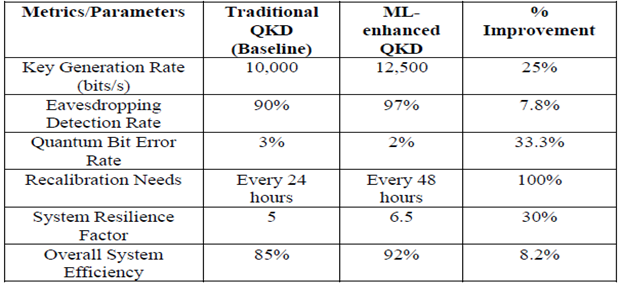
\includegraphics[scale=0.65]{qkd.png}}
	\label{table5}
\end{table}

\section{Study Results}
The remarkable power of quantum computers in parallel information processing suggests that the use of these types of computers in machine learning could be highly beneficial. Wherever machine learning (ML) is applicable, quantum machine learning (QML) is also relevant, often leading to improvements in efficiency, accuracy, and faster learning processes. It is noteworthy that all these results have been achieved with NISQ-era quantum computers, which are considered as weak quantum computers. This indicates that with advancements in technology and improvements in these computers, significant breakthroughs could be realized. However, it should not be overlooked that quantum computers also have their limitations. Constructing quantum computers is a very challenging and costly endeavor, and the existing computers are often accompanied by noise and have a limited number of qubits.

\section{Conclusion}
In this research, we provided a brief history of the development of quantum computing technology and quantum machine learning. We become familiar with the concepts of qubits, entanglement, superposition, and the power of processing which these computers offer. We also explored quantum gates and circuits, understanding the components that make up quantum algorithms. Finally, by examining the applications of quantum machine learning across various fields, we observed that, despite its limitations, quantum machine learning has made significant advancements. We also noted that the models presented in the research have plenty of room for improvement, indicating a promising future for this area of technology. With such results from experiments, it is expected that quantum technologies, including quantum machine learning, will have a substantial impact in the near future and make significant contributions to diverse fields of science.


\begin{thebibliography}{00}
\bibitem{b1} N. T. Singh, A. Swetapadma, and P. K. Pattnaik, “A Comparative Study of Quantum Machine Learning Enhanced SVM and Classical SVM for Brain Stroke Prediction,” in 2023 International Conference on Computer Communication and Informatics (ICCCI), Coimbatore, India: IEEE, Jan. 2023, pp. 1–4. doi: 10.1109/ICCCI56745.2023.10128293.
\bibitem{b2} P. Kuppusamy, N. Yaswanth Kumar, J. Dontireddy, and C. Iwendi, “Quantum Computing and Quantum Machine Learning Classification – A Survey,” in 2022 IEEE 4th International Conference on Cybernetics, Cognition and Machine Learning Applications (ICCCMLA), Goa, India: IEEE, Oct. 2022, pp. 200–204. doi: 10.1109/ICCCMLA56841.2022.9989137.
\bibitem{b3} S. Garg and G. Ramakrishnan, “Advances in Quantum Deep Learning: An Overview.” arXiv, May 08, 2020. doi: 10.48550/arXiv.2005.04316.
\bibitem{b4} R. Ur Rasool, H. F. Ahmad, W. Rafique, A. Qayyum, J. Qadir, and Z. Anwar, “Quantum Computing for Healthcare: A Review,” Future Internet, vol. 15, no. 3, Art. no. 3, Mar. 2023, doi: 10.3390/fi15030094.
\bibitem{b5} M. T. N, A. Hiremath, N. M, S.-L. Peng, S. M. R, and P. S. K, “A Survey on Machine Learning Techniques Using Quantum Computing,” in 2022 Fourth International Conference on Emerging Research in Electronics, Computer Science and Technology (ICERECT), Mandya, India: IEEE, Dec. 2022, pp. 1–6. doi: 10.1109/ICERECT56837.2022.10059764.
\bibitem{b8} J. D. Hidary, “A Brief History of Quantum Computing,” in Quantum Computing: An Applied Approach, J. D. Hidary, Ed., Cham: Springer International Publishing, 2021, pp. 15–21. doi: 10.1007/978-3-030-83274-2\_2.
\bibitem{b9} L. K. Grover, “A fast quantum mechanical algorithm for database search.” arXiv, Nov. 19, 1996. doi: 10.48550/arXiv.quant-ph/9605043.
\bibitem{b10} N. Wiebe, D. Braun, and S. Lloyd, “Quantum Data Fitting,” Phys. Rev. Lett., vol. 109, no. 5, p. 050505, Aug. 2012, doi: 10.1103/PhysRevLett.109.050505.
\bibitem{b11} A. W. Harrow, A. Hassidim, and S. Lloyd, “Quantum Algorithm for Linear Systems of Equations,” Phys. Rev. Lett., vol. 103, no. 15, p. 150502, Oct. 2009, doi: 10.1103/PhysRevLett.103.150502.
\bibitem{b12} E. Farhi and H. Neven, “Classification with Quantum Neural Networks on Near Term Processors.” arXiv, Aug. 30, 2018. doi: 10.48550/arXiv.1802.06002.
\bibitem{b13} J. Biamonte, P. Wittek, N. Pancotti, P. Rebentrost, N. Wiebe, and S. Lloyd, “Quantum Machine Learning,” Nature, vol. 549, no. 7671, pp. 195–202, Sep. 2017, doi: 10.1038/nature23474.
\bibitem{b14} S. Jain, A. Gandhi, S. Singla, L. Garg, and S. Mehla, “Quantum Machine Learning and Quantum Communication Networks: The 2030s and the Future,” in 2022 International Conference on Computational Modelling, Simulation and Optimization (ICCMSO), Pathum Thani, Thailand: IEEE, Dec. 2022, pp. 59–66. doi: 10.1109/ICCMSO58359.2022.00025.
\bibitem{b15} S. N. Pushpak and S. Jain, “An Introduction To Quantum Machine Learning Techniques,” in 2021 9th International Conference on Reliability, Infocom Technologies and Optimization (Trends and Future Directions) (ICRITO), Noida, India: IEEE, Sep. 2021, pp. 1–6. doi: 10.1109/ICRITO51393.2021.9596240.
\bibitem{b16} S. N. Pushpak and S. Jain, “An Implementation of Quantum Machine Learning Technique to Determine Insurance Claim Fraud,” in 2022 10th International Conference on Reliability, Infocom Technologies and Optimization (Trends and Future Directions) (ICRITO), Noida, India: IEEE, Oct. 2022, pp. 1–5. doi: 10.1109/ICRITO56286.2022.9964828.
\bibitem{b17} R. Bhavsar et al., “Classification of Potentially Hazardous Asteroids Using Supervised Quantum Machine Learning,” IEEE Access, vol. 11, pp. 75829–75848, 2023, doi: 10.1109/ACCESS.2023.3297498.
\bibitem{b18} B. E. Baaquie and L.-C. Kwek, “Quantum Superposition and Entanglement,” in Quantum Computers: Theory and Algorithms, B. E. Baaquie and L.-C. Kwek, Eds., Singapore: Springer Nature, 2023, pp. 107–130. doi: 10.1007/978-981-19-7517-2\_5.
\bibitem{b19} A. Jhanwar and M. J. Nene, “Enhanced Machine Learning using Quantum Computing,” in 2021 Second International Conference on Electronics and Sustainable Communication Systems (ICESC), Coimbatore, India: IEEE, Aug. 2021, pp. 1407–1413. doi: 10.1109/ICESC51422.2021.9532638.
\bibitem{b20} L. S. W. III, Essential Mathematics for Quantum Computing: A beginner’s guide to just the math you need without needless complexities. Packt Publishing Ltd, 2022.
\bibitem{b21} Y. Kwak, W. J. Yun, S. Jung, J.-K. Kim, and J. Kim, “Introduction to Quantum Reinforcement Learning: Theory and PennyLane-based Implementation,” in 2021 International Conference on Information and Communication Technology Convergence (ICTC), Oct. 2021, pp. 416–420. doi: 10.1109/ICTC52510.2021.9620885.
\bibitem{b22} S. K. Sood and Pooja, “Quantum Computing Review: A Decade of Research,” IEEE Transactions on Engineering Management, vol. 71, pp. 6662–6676, 2024, doi: 10.1109/TEM.2023.3284689.
\bibitem{b23} A. Senokosov, A. Sedykh, A. Sagingalieva, B. Kyriacou, and A. Melnikov, “Quantum machine learning for image classification,” Mach. Learn.: Sci. Technol., vol. 5, no. 1, p. 015040, Mar. 2024, doi: 10.1088/2632-2153/ad2aef.
\bibitem{b24} J.-R. Jiang, “A Quick Overview of Quantum Machine Learning,” in 2023 IEEE 5th Eurasia Conference on IOT, Communication and Engineering (ECICE), Yunlin, Taiwan: IEEE, Oct. 2023, pp. 301–304. doi: 10.1109/ECICE59523.2023.10383149.
\bibitem{b25} M. Esposito, G. Uehara, and A. Spanias, “Quantum Machine Learning for Audio Classification with Applications to Healthcare,” in 2022 13th International Conference on Information, Intelligence, Systems \& Applications (IISA), Jul. 2022, pp. 1–4. doi: 10.1109/IISA56318.2022.9904377.
\bibitem{b26} M. Abbaszade, V. Salari, S. S. Mousavi, M. Zomorodi, and X. Zhou, “Application of Quantum Natural Language Processing for Language Translation,” IEEE Access, vol. 9, pp. 130434–130448, 2021, doi: 10.1109/ACCESS.2021.3108768.
\bibitem{b27} G. Nagaraj, N. Upadhayaya, A. Matroud, N. Sabitha, R. V.K, and R. Nagaraju, “A Detailed Investigation on Potential Impact of Quantum Computing on Improving Artificial Intelligence,” in 2023 International Conference on Innovative Data Communication Technologies and Application (ICIDCA), Mar. 2023, pp. 447–452. doi: 10.1109/ICIDCA56705.2023.10099821.
\bibitem{b28} G. Li, X. Zhao, and X. Wang, “Quantum self-attention neural networks for text classification,” Sci. China Inf. Sci., vol. 67, no. 4, p. 142501, Mar. 2024, doi: 10.1007/s11432-023-3879-7.
\bibitem{b29} U. Ullah and B. Garcia-Zapirain, “Quantum Machine Learning Revolution in Healthcare: A Systematic Review of Emerging Perspectives and Applications,” IEEE Access, vol. 12, pp. 11423–11450, 2024, doi: 10.1109/ACCESS.2024.3353461.
\bibitem{b30} B. R.M, M. Nalini, N. Vijayaraj, and A. M. J. Kinol, “Enhancing Quantum Key Distribution Protocols with Machine Learning Techniques,” in 2023 Intelligent Computing and Control for Engineering and Business Systems (ICCEBS), Dec. 2023, pp. 1–4. doi: 10.1109/ICCEBS58601.2023.10448811.
\bibitem{b31} D. Quiroga, P. Date, and R. Pooser, “Discriminating Quantum States with Quantum Machine Learning,” in 2021 IEEE International Conference on Quantum Computing and Engineering (QCE), Oct. 2021, pp. 481–482. doi: 10.1109/QCE52317.2021.00088.
\bibitem{b32} S. Y.-C. Chen, C.-M. Huang, C.-W. Hsing, H.-S. Goan, and Y.-J. Kao, “Variational quantum reinforcement learning via evolutionary optimization,” Mach. Learn.: Sci. Technol., vol. 3, no. 1, p. 015025, Feb. 2022, doi: 10.1088/2632-2153/ac4559.
\bibitem{b33} S. Lokes, C. S. J. Mahenthar, S. P. Kumaran, P. Sathyaprakash, and V. Jayakumar, “Implementation of Quantum Deep Reinforcement Learning Using Variational Quantum Circuits,” in 2022 International Conference on Trends in Quantum Computing and Emerging Business Technologies (TQCEBT), Oct. 2022, pp. 1–4. doi: 10.1109/TQCEBT54229.2022.10041479.
\bibitem{b34} L. Lamata, “Quantum Reinforcement Learning with Quantum Photonics,” Photonics, vol. 8, no. 2, Art. no. 2, Feb. 2021, doi: 10.3390/photonics8020033.
\bibitem{b36} H. Xiong, X. Duan, Y. Yu, J. Zhang, and H. Yin, “Image Classification Based on Quantum Machine Learning,” in 2023 5th International Conference on Intelligent Control, Measurement and Signal Processing (ICMSP), Chengdu, China: IEEE, May 2023, pp. 891–895. doi: 10.1109/ICMSP58539.2023.10170998.
\bibitem{b37} A. Senokosov, A. Sedykh, A. Sagingalieva, B. Kyriacou, and A. Melnikov, “Quantum machine learning for image classification,” Mach. Learn.: Sci. Technol., vol. 5, no. 1, p. 015040, Mar. 2024, doi: 10.1088/2632-2153/ad2aef.
\bibitem{b38} J. Kim, “Quantum Federated Learning for Vehicular Computing Scenarios,” in 2023 14th International Conference on Information and Communication Technology Convergence (ICTC), Oct. 2023, pp. 168–172. doi: 10.1109/ICTC58733.2023.10392753.
\end{thebibliography}

\end{document}
